\documentclass[thesis.tex]{subfiles}

\begin{document}
\chapter{Performance testing}
This chapter is concerned with testing the efficiency of the approach by running tests on the implemented tool. There are two metrics which will be presented: The running time of the algorithm and the correctness of the result. How correctness is determined is covered in section \ref{sec:performance_validation}. Most of the results are compared against running the same alignment with an own PO-MSA implementation. PO-MSA is chosen because of its intuitive nature, the easily deducible relationship between graph complexity and running time, and, most importantly, because it is not a heuristical approach which means it guarantees a correct result every time.
\section{Test data}
These tests are meant to reflect usage in a what would be an every day situation, and does therefore use real genetic data. All of the sequences are FASTA-files from the MHC region, most fetched from the vg github repo\cite{vg}, some from the test-set provided by the sequence graphs tool\cite{sequence_graphs}. The exact test sets are chosen to provide a variety of sequence lengths. In order to cover lengths where we found no sequences there are created artificial sequences by cutting out suitable regions from longer sequences. All the sequences which are used can be found in the test-folder of the github repo of the tool (Appendix \ref{sec:tool}).\\
\par\noindent
There are exactly 6 data-sets involved in the testing:
\begin{itemize}
  \item mhc1.fa
\end{itemize}
In the following tests the data sets are referenced by their given name only.\\
\par\noindent
In order to do alignments we needed reads aswell as the reference data itself. These reads are generated by the read-generator seen in the appendix. A read $r$ from a graph $G$ is generated by the following procedure:
\begin{enumerate}
  \item Choose a random vertice $v \in G\{s_G, t_G\}$ such that the smallest distance from $v$ to $t_g$ is larger than the chosen read size $|r|$
  \item For $r$ steps:
  \begin{enumerate}
    \item Append $b(v_x)$ to the read $r$
    \item Choose a random neighbouring vertice $v_y \in neighbours(v_x)$ as the new $v_x$
  \end{enumerate}
  \item for $r_i \in r$
  \begin{enumerate}
    \item Choose a random floating point value $0<=v<=1$
    \begin{itemize}
      \item If $v<p$ delete $r_i$
      \item Else if $v<2p$ add a random base $b \in \{A, C, G, T\}$ before $r_i$
      \item Else if $v<3p$ substitue $r_i$ with a random base $b \in \{A, C, G, T\} \\ \{r_i\}$
    \end{itemize}
  \end{enumerate}
  \item Output $r$
\end{enumerate}
In order to provide reproducability the randomness in the reads are generated from a seed found in the ReadGenerator tool.\\
\par\noindent
Because this thesis is concerned with the mathematical properties of the model the noise in the reads does not necessarily depict the true nature of either genetic variation (Section \ref{sec:genetic_variation}) or read errors (Section \ref{sec:sequencing}). In the graph domain determining the errors of a read corresponds to determining which path the read originates from. For the cases where this does not directly correspond to finding the highest scoring path this is an impossible task without more information (such as other aligned reads), and the work is thus left for others. 
\section{Validation}
\label{sec:performance_validation}
When an alignment is produced for a read we classify it as either as correct or not correct. Intuitively one could imagine this can be determined by whether the generated read aligns back to the path it was generated from. However, when noise is introduced an interesting phenomenon can occur: The modified read can be more similar to another path in the graph than its origin. This can also occur whenever there exists actual equal paths in the graph, typically in the case of repeats. In order to stick with mathemathical properties, optimality holds no relation to the origin of a read but is purely defined as the path which produces the highest possible alignment score. As PO-MSA is an exhaustive search we define optimally aligned as alignments which produce the same alignment score as the highest score found by PO-MSA. Consequently, as only the scores are compared, even when the approach produces a different alignments than PO-MSA this can be classified as optimal.
\section{Time capturing mechanisms}
For both the "Fuzzy context-based search" and the PO-MSA algorithm the time capturing mechanisms are built into the tool, using the Java System object. This allowed us to wrap the time capturing of each individual constituent as close to the functional parts as possible in order to avoid unecessary overhead. When comparing tools the time was taken from the tool was started until the tool ended. Doing it this way has several disadvantages, which are discussed in Section \ref{sec:comparison_tools}.
\section{Building the index}
\begin{wraptable}{r}{0.5\textwidth}
  \begin{tabular}{|l|r|r|}
    \hline \textbf{Data set:} & \textbf{$|G|$} & \textbf{Time (ms)}\\ \hline
    mhc1.fa & 701 & 597127\\ \hline
    primary.fasta & 3416 & 2050636\\ \hline
    20k.fasta & 20931 & 13858701\\ \hline
    30k.fasta & 37801 & 25401423\\ \hline
    100k.fasta & 100351 & 77928851\\ \hline
    150k.fa & 152451 & 122654330\\ \hline
  \end{tabular}
  \caption{Runtimes of build\_index.sh}
\end{wraptable}
The building of the index is the first step of the process realized through the build\_index.sh script. To summarize this step consists of reading the input files, building the graph and generating the suffix trees. The build process was run 50 times on 6 different data sets, the averaged results can be seen in table \ref{tab:build_index}. All of these are linear operations, and a linear trend can clearly be seen in figure \ref{build_index}.\\
\begin{figure}[!b]
    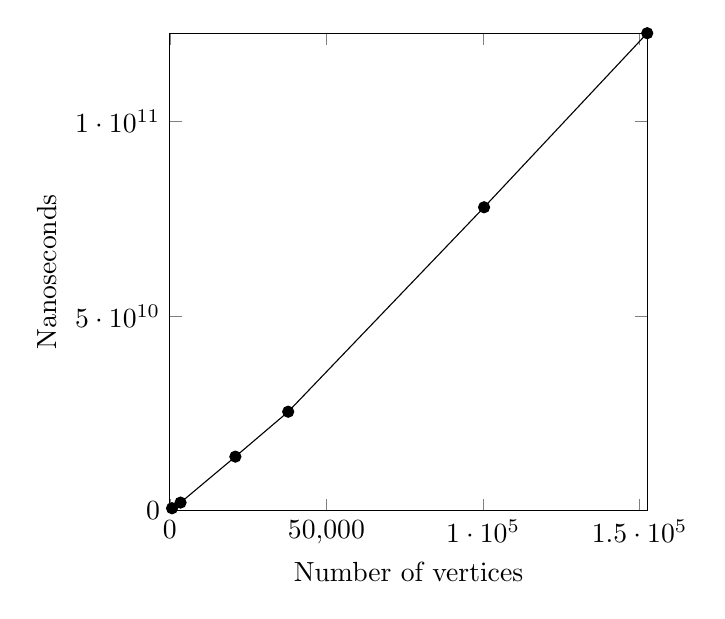
\begin{tikzpicture}
      \begin{axis}[scale only axis,height=0.5\textwidth,width=0.5\textwidth,xmin=0,ymin=0,xmax=152451,ymax=122654330941,scaled ticks=false, xlabel={Number of vertices}, ylabel={Nanoseconds}, max space between ticks=50pt]
        \addplot[color=black,mark=*] coordinates {
          (701,597127494)
          (3416,2050636347)
          (20931,13858701254)
          (37801,25401423058)
          (100351,77928851412)
          (152451,122654330941)
        };
      \end{axis}
    \end{tikzpicture}
    \caption{Runtime for the build index procedure}
    \label{fig:build_index}
\end{figure}
\clearpage
\noindent
When splitting up the runtime into the individual constituents an interesting pattern emerges (Fig. \ref{fig:index_constituents}): The main load of the indexation lies in writing to file. The data structure used is a large tree of nested complex structures like hashmaps, which the standard Java serialization does not handle well \textcolor{red}{PROB SHUD REFERENCE SOMETHING. API MAYBE}. Putting effort into reducing the size of the index will thus have a dramatic effect on the time complexity.
\begin{figure}[!t]
  \begin{subfigure}[t]{0.4\textwidth}
    \begin{tikzpicture}[trim axis left]
      \begin{axis}[scale only axis,height=\textwidth,width=\textwidth,xmin=0,ymin=0,xmax=152451,ymax=122654330941,scaled ticks=false]
        \addplot coordinates {
          (701,9404263)
          (3416,51489024)
          (20931,623903806)
          (37801,1031820116)
          (100351,5487825644)
          (152451,11328920839)
        };
      \end{axis}
    \end{tikzpicture}
    \subcaption{Time used building the graph}
  \end{subfigure}
  \hfill
  \begin{subfigure}[t]{0.4\textwidth}
    \begin{tikzpicture}[trim axis left]
      \begin{axis}[scale only axis,height=\textwidth,width=\textwidth,xmin=0,ymin=0,xmax=152451,ymax=122654330941,scaled ticks=false]
        \addplot[color=green,mark=*] coordinates {
          (701,65184733)
          (3416,138556745)
          (20931,269431681)
          (37801,2788165703)
          (100351,6905517064)
          (152451,10007919085)
        };
      \end{axis}
    \end{tikzpicture}
    \subcaption{Time used building the index}
  \end{subfigure}
  \begin{subfigure}[b]{0.4\textwidth}
    \begin{tikzpicture}[trim axis left]
      \begin{axis}[scale only axis,height=\textwidth,width=\textwidth,xmin=0,ymin=0,xmax=152451,ymax=122654330941,scaled ticks=false]
        \addplot[color=red,mark=*] coordinates {
          (701,522174790)
          (3416,1860265733)
          (20931,1296505592)
          (37801,21581107294)
          (100351,65535179527)
          (152451,101317180800)
        };
      \end{axis}
    \end{tikzpicture}
    \subcaption{Time used writing the index\vspace{\baselineskip}}
  \end{subfigure}
  \hfill
  \begin{subfigure}[b]{0.4\textwidth}
  \begin{tikzpicture}[trim axis left]
    \begin{axis}[scale only axis,height=\textwidth,width=\textwidth,xmin=0,ymin=0,xmax=152451,ymax=122654330941,scaled ticks=false]
      \addplot[name path=axis] coordinates {
        (0, 0)
        (152451, 0)
      };
      \addplot[color=blue,name path=graph] coordinates {
        (701,9404263)
        (3416,51489024)
        (20931,623903806)
        (37801,1031820116)
        (100351,5487825644)
        (152451,11328920839)
      };
      \addplot[color=green, name path=index] coordinates {
        (701,9404263 + 65184733)
        (3416,51489024 + 138556745)
        (20931,6239033806 + 269431681)
        (37801,1031820116 + 2788165703)
        (100351,5487825644 + 6905517064)
        (152451,11328920839 + 10007919085)
      };
      \addplot[color=black, name path=total,mark=*] coordinates {
        (701,597127494)
        (3416,2050636347)
        (20931,13858701254)
        (37801,25401423058)
        (100351,77928851412)
        (152451,122654330941)
      };
      \addplot[red!30] fill between[of=index and total];
      \addplot[green!30] fill between[of=graph and index];
      \addplot[blue!30] fill between[of=graph and axis];
    \end{axis}
  \end{tikzpicture}
  \subcaption{Total run time as a combination of the individual steps}
  \end{subfigure}
  \caption{Time (ns) used by the indexation process as a function of the number of vertices}
  \label{fig:index_constituents}
\end{figure}
\section{Alignment}
The alignment tests are run by the align\_sequence.sh script, both with \texttt{--type=fuzzy} and \texttt{--type=po\_msa} flags. The section is divided into segments, based on what variable is tuned. As a remainder to the reader, these are the variables which are in play:
\begin{itemize}
  \item $|G|$ is the size of the graph
  \item $\lambda$ is the allowed error margin
  \item $|s|$ is the length of the input sequence
  \item $b$ is the branching factor of the graph
\end{itemize}
Additionally we include one more variable:
\begin{itemize}
  \item $p$ is the amount of noise added to the reads
\end{itemize}
Each section is concerned the impact of exactly one of these variables, so all the other ones are locked to a value for the entirety of the run. Some of the variables, such as $\lambda$, does not exist in the PO-MSA alignment procedure. In these cases the PO-MSA result is shown as a constant function, representing a single set of runs.\\
\par\noindent
The tests are run on the same datasets as in the previous section. Each of the two types of alignment approaches are ran 50 times, when runtimes are discussed this is as an average over all the run. The onlye variable which is not tested explicitly is $|c|$ which is automatically set by the tool in all the test runs.
\subsection*{Runtime as a function of graph size\\
($|G|=x$, $\lambda=0$, $|s|=100$, $b=1$, $p=0.0$)}
During the introduction in section \ref{sec:po_msa}, PO-MSA was said to be vulnerable in regards to graph complexity. The pure number of vertices is one of the factors making up this complexity. As expected the time usage of PO-MSA is very linear with regards to the graph size (Fig. \ref{runtime_G}). The time spent by the fuzzy algorithm seems constant in comparison. As the number of vertices only affect the context length in an extremely logarithmic way, and this length decides the depth of the suffix tree search this makes sense.
\begin{figure}
  \begin{tikzpicture}
    \begin{axis}[scale only axis,height=\textwidth,width=\textwidth,xmin=0,ymin=0,xmax=152451,ymax=5000000000,scaled ticks=false, legend pos=north west, xlabel={$|G|$}, ylabel={Nanoseconds}]
      \addplot[color=blue,mark=*] coordinates {
        (701, 28197210)
        (3416, 32719710)
        (20931, 33308335)
        (37801,  30339892)
        (100351, 41266794)
        (152451, 55771208)
      };
      \addplot[color=black,mark=*] coordinates {
        (701, 50715055)
        (3416, 106071102)
        (20931, 331411927)
        (37801,  817322537)
        (100351, 2521874503)
        (152451, 2741174182)
      };
      \addlegendentry{Fuzzy}
      \addlegendentry{PO-MSA}
    \end{axis}
  \end{tikzpicture}
  \caption{Runtime of the alignment process as a function of $|G|$}
  \label{fig:runtime_G}
\end{figure}
\subsection*{Runtime as a function of error margin\\
($|G|=500.000$, $\lambda=x$, $|s|=100$, $b=1$, $p=0.0$)}
\begin{figure}
  \begin{tikzpicture}
    \begin{axis}[scale only axis,height=\textwidth,width=\textwidth,xmin=0,ymin=0,xmax=5,ymax=6000000000,scaled ticks=false, legend pos=north west, xlabel={$\lambda$}, ylabel={Nanoseconds},xtick={0,1,2}]
      \addplot[color=blue,mark=*] coordinates {
        (0, 54895773)
        (1, 399468059)
        (2, 5059148546)
      };
      \addplot[color=black,mark=*] coordinates {
        (0, 2008561551)
        (5, 2008561551)
      };
      \addplot[dashed] coordinates {
      }
      \addlegendentry{Fuzzy}
      \addlegendentry{PO-MSA}
      \addlegendentry{Correctly mapped reads}
    \end{axis}
    \begin{axis}[scale only axis,height=\textwidth,width=\textwidth,
      xmin=0,xmax=5,
      ymin=0,ymax=100,
      axis y line*=right,
      ylabel={Percentage of correctly mapped reads}
      xtick={0,1,2,3,4,5},
      xticklabels={,,,,,}]
      \addplot[dashed] coordinates {
        (0, (28/50)*100)
        (1, 19/50*100)
        (2, 0)
      };
    \end{axis}
  \end{tikzpicture}
  \caption{Runtime of the alignment process as a function of $\lambda$}
  \label{fig:runtime_lambda}
\end{figure}
\subsection*{Runtime as a function of sequence length\\
($|G|=500.000$, $\lambda=0$, $|s|=x$, $b=1$, $p=0.0$)}
\subsection*{Runtime as a function of graph complexity\\
($|G|=500.000$, $\lambda=0$, $|s|=100$, $b=x$, $p=0.0$)}
\subsection*{Runtime as a function of noise\\
($|G|=500.000$, $\lambda=0$, $|s|=100$, $b=1$, $p=x$)}
\section{Comparison with other tools}
\label{sec:comparison_tools}
\end{document}